\subsection{Background and Impact}


Many of the recent, most celebrated successes of artificial intelligence (AI), such as AlphaStar~\cite{starcraft2019}, AlphaGo~\cite{silver2017mastering}, OpenAI Five~\cite{berner2019dota}, and their derivative systems~\cite{alphazero}, utilize deep reinforcement learning to achieve human or super-human level performance in sequential decision-making tasks.
%As established by~\citet{amodei_hednandez_2018}, these improvements to the state-of-the-art have thus far required exponentially increasing computational power to achieve such performance.
    These improvements to the state-of-the-art have thus far required exponentially increasing computational power to achieve such performance~\cite{amodei_hednandez_2018}.
        In part, this is due to an increase in the computation required per environment-sample; however, the most significant change is the number of environment-samples required for training. 
            For example, DQN~\cite{mnih2015human}, A3C~\cite{mnih2016asynchronous}, and Rainbow DQN~\cite{hessel2018rainbow} have been applied to ATARI 2600 games~\cite{bellemare2013arcade} and require from 44 to over 200 million frames (200 to over 900 hours) to achieve human-level performance. 
            On more complex domains: OpenAI Five utilizes 11,000+ years of Dota 2 gameplay~\cite{openai_2018}, AlphaGoZero uses 4.9 million games of self-play in Go~\cite{silver2017mastering}, and AlphaStar uses 200 years of StarCraft~II gameplay~\cite{deepmind}. 
    Due to the growing computational requirements, a shrinking portion of the AI community has the resources to improve these systems and reproduce state-of-the-art results. 
        Additionally, the application of many reinforcement learning techniques to real-world challenges, such as self-driving vehicles, is hindered by the raw number of required samples.
        In these real-world domains, policy roll-outs can be costly and simulators are not yet accurate enough to yield policies robust to real-world conditions.

One well-known way to reduce the environment sample-complexity of the aforementioned methods is to leverage human priors and demonstrations of the desired behavior. 
    Techniques utilizing trajectory examples, such as imitation learning and Bayesian reinforcement learning, have been successfully applied to older benchmarks and real-world problems where samples from the environment are costly.  
        In many simple games with singular tasks, such as the Atari 2600~\cite{bellemare2013arcade}, OpenAI Gym~\cite{gym}, and TORCS environments\footnote{\url{https://github.com/ugo-nama-kun/gym_torcs}}, imitation learning can drastically reduce the number of environment samples needed through pretraining and hybrid RL techniques~\cite{cruz2017pre,gao2018reinforcement,hester2018deep,panse2018imitation}.
        Further, in some real-world tasks, such as robotic manipulation~\cite{finn2016guided,finn2017one} and self-driving~\cite{bojarski2016end}, in which it is expensive to gather a large number of samples from the environment, imitation-based methods are often the only means of generating solutions using few samples.
    Despite their success, these techniques are still not sufficiently sample-efficient for application to many real-world domains. 


\begin{figure}
    \centering
    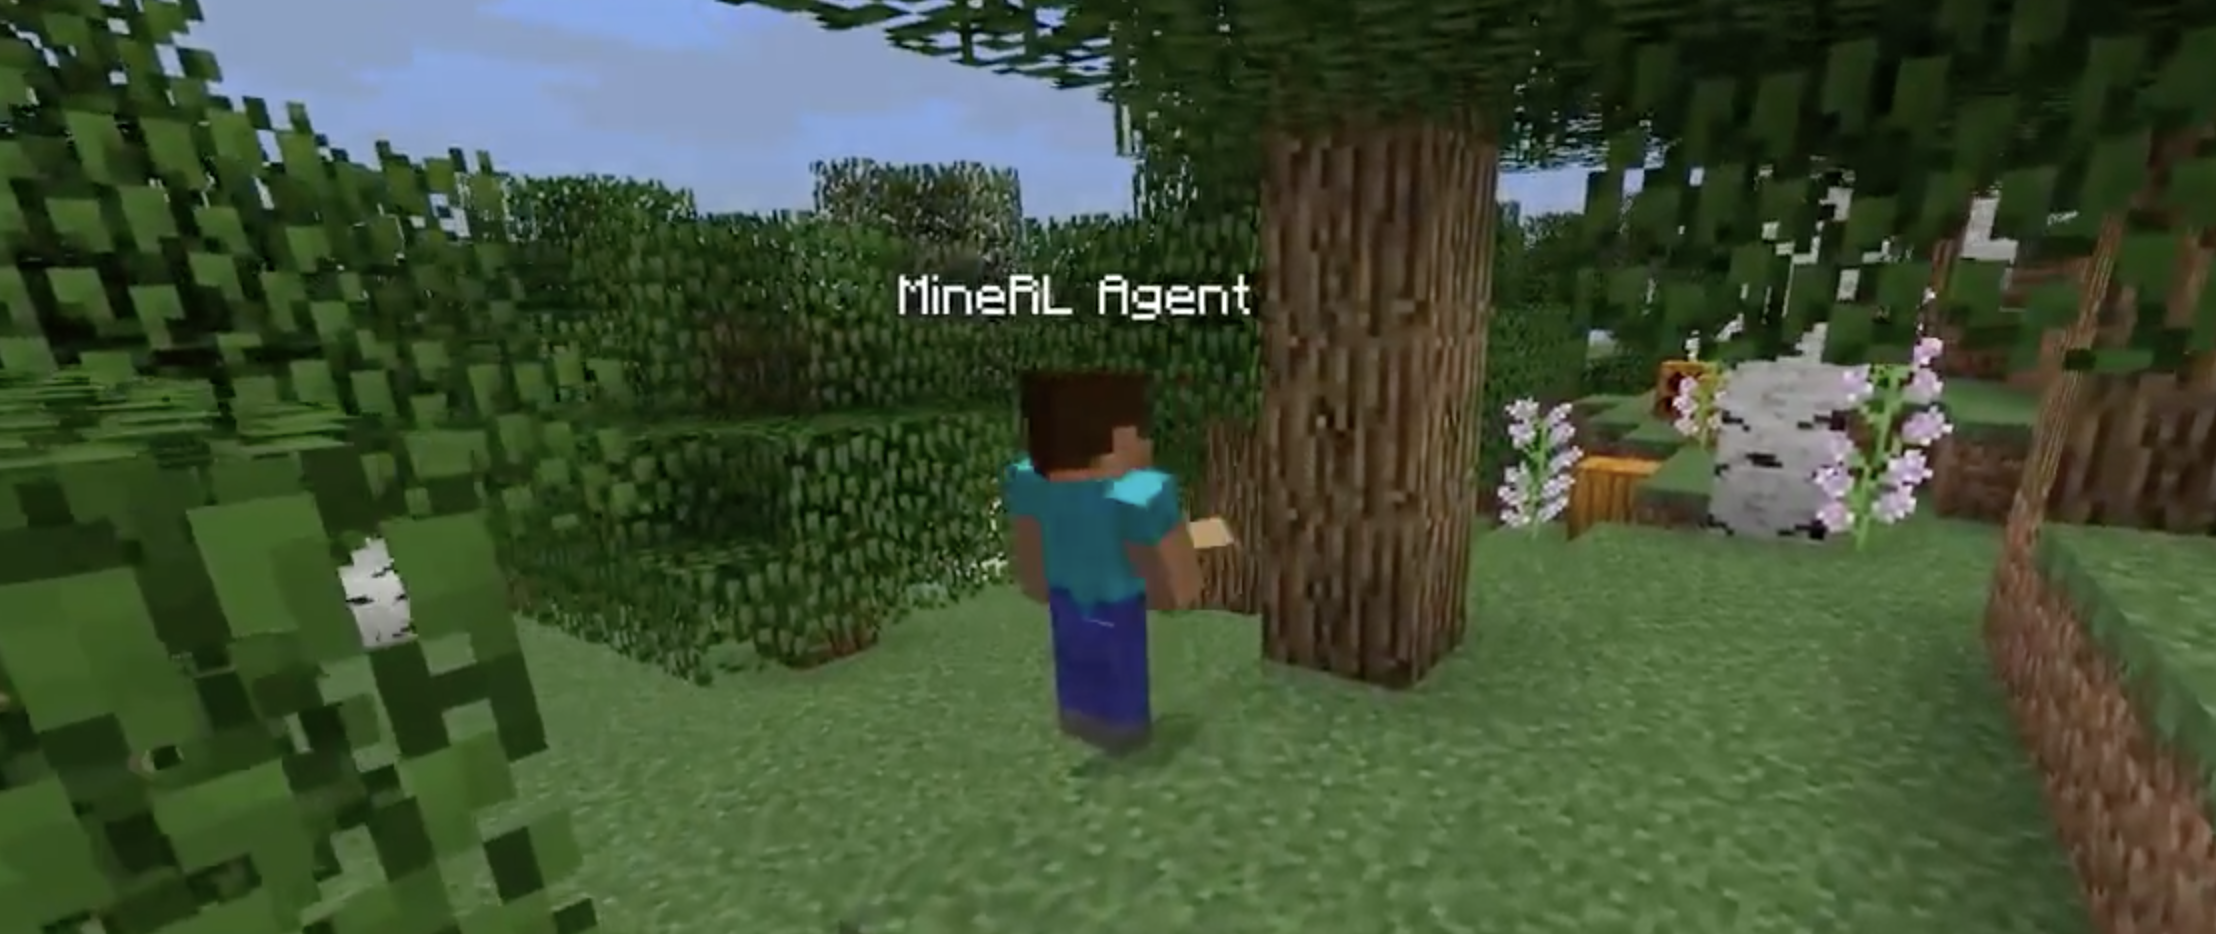
\includegraphics[width=0.8\textwidth]{assets/2019.png}
    \caption{\small{The top agent from the MineRL 2019 competition mining the first item required to eventually obtain a diamond.}}
\end{figure}

\paragraph{Impact.} To that end, the central aim of our proposed competition is the advancement and development of novel, sample-efficient methods which leverage human priors for sequential decision-making problems. 
    Due to the competition's design, organizational team, and support, we are confident that the competition will catalyze research towards the deployment of reinforcement learning in the real world, democratized access to AI/ML, and reproducibility. 
    By enforcing constraints on the computation and sample budgets of the considered techniques, we believe that the methods developed during the competition will broaden participation in deep RL research by lowering the computational barrier to entry. 

% barrier-to-entry reduction 
While computational resources inherently have a cost barrier, large-scale, open-access datasets can be widely used. 
    To that end, we center our proposed competition around techniques which leverage the \minenet{} dataset~\cite{gussminerlijcai2019}.
    To maximize the development of domain-agnostic techniques that enable the application of deep reinforcement learning to sample-limited, real-world domains, such as robotics, we carefully developed a novel data-pipeline and hold-out environment evaluation scheme with AIcrowd to prevent the over-engineering of submissions to the competition task.

% Research impact stimulating methods.
Crucially, the competition will stimulate a broad set of new techniques in reinforcement and imitation learning. 
    In the previous NeurIPS 2019 iteration of the competition, competitors developed several new algorithms and approaches to tackle the challenge in spite of the difficult sample-complexity limitations~\cite{gussminerlneurips2019}.
        Ranging from hierarchical imitation methods to novel inverse reinforcement learning techniques, the research impact of the competition was broad in scope, yielding a diverse set of solutions~\cite{milani2020minerl}. 
    With the addition of new competition features and refined submission and evaluation pipelines (see Section~\ref{sec:novelty}),
    we anticipate this year's competition to garner further research progress of relevance to the NeurIPS community.

Our competition will further attract a large number of participants from within and outside of the NeurIPS community. 
    Given the broad interest and participation in the previous year (attracting over 1000 registered participants with a total of 662 full submissions\footnote{\url{https://www.aicrowd.com/challenges/neurips-2019-minerl-competition}}), our extensive media coverage~\cite{hsu_2019,shead_2019,synced_2019,vincent_2019}, and improvements to user-experience, we expect the number of participants to grow to 1300 users and the number of successful submission to increase to over 1000 agents. To effectuate this growth, we will deliver several improvements over prior years. First, we plan to drastically simplify the submission process and provide thorough multi-media documentation to increase the conversion-rate from registration to submission. Further, we intend on providing more compelling visualizations for the competitors' submissions, generating external interest from outside of the research community. Expanding on media coverage and outreach channels from last year, we will utilize mailing lists and social media announcements to retain the previous competitor pool and expand our user-base to new demographics.
        Moreover, the expansion of our competition to multiple tracks supporting pure imitation learning and hybridized imitation and reinforcement learning submissions will broaden the the appeal of our competition as a vehicle for researching and developing new methods.


The proposed competition is ambitious, so we have taken meaningful steps to ensure its smooth execution. 
Specifically, we are currently securing several crucial partnerships with organizations and individuals. 
During the MineRL 2019 competition, our primary partner, Microsoft Research, provided significant computational resources to enable direct, fair evaluation of the participants' training procedures. 
We developed a relationship with AIcrowd to provide the submission orchestration platform for our competition, as well as continued support throughout the competition to ensure that participants can easily submit their algorithms. Additionally, we partnered with Preferred Networks in the previous iteration of this competition to provide a set of standard baseline implementations, which include many state of the art reinforcement learning and imitation learning techniques. By leveraging our previous partnerships and developing new ones, we expect to largely increase the scale, success, and impact of the competition.


% The recent proliferation of machine learning and artificial intelligence (ML/AI) systems has deep implications for our society's structure; as automation subsumes human labor in many industrial sectors, those with the means to develop and deploy these new systems stand to profit, while those without are displaced and disenfranchised~\cite{groshen2018preparing}. 
% This trend will have a disproportionate effect on economically disadvantaged communities~\cite{west2015happens, algernon_bucknor_rockeymoore_2017, groshen2018preparing}. 
% A primary mechanism through which this inequality materializes is the growing \emph{computational barrier to entry:}  % (see Figure [\todo{add cool fig}]). 
% In turn, these systems have been largely developed by institutions with substantial research grants or by corporations able to justify the cost of development (computation) due to subsequent wide-spread use.
% Unless direct steps are taken to democratize these AI/ML systems by addressing their growing computational inaccessibility, a limited number of institutions will likely continue to be the majority participants in their development. 
% \newpage


\subsubsection{Domain Interest}

\begin{figure}
    \begin{center}
        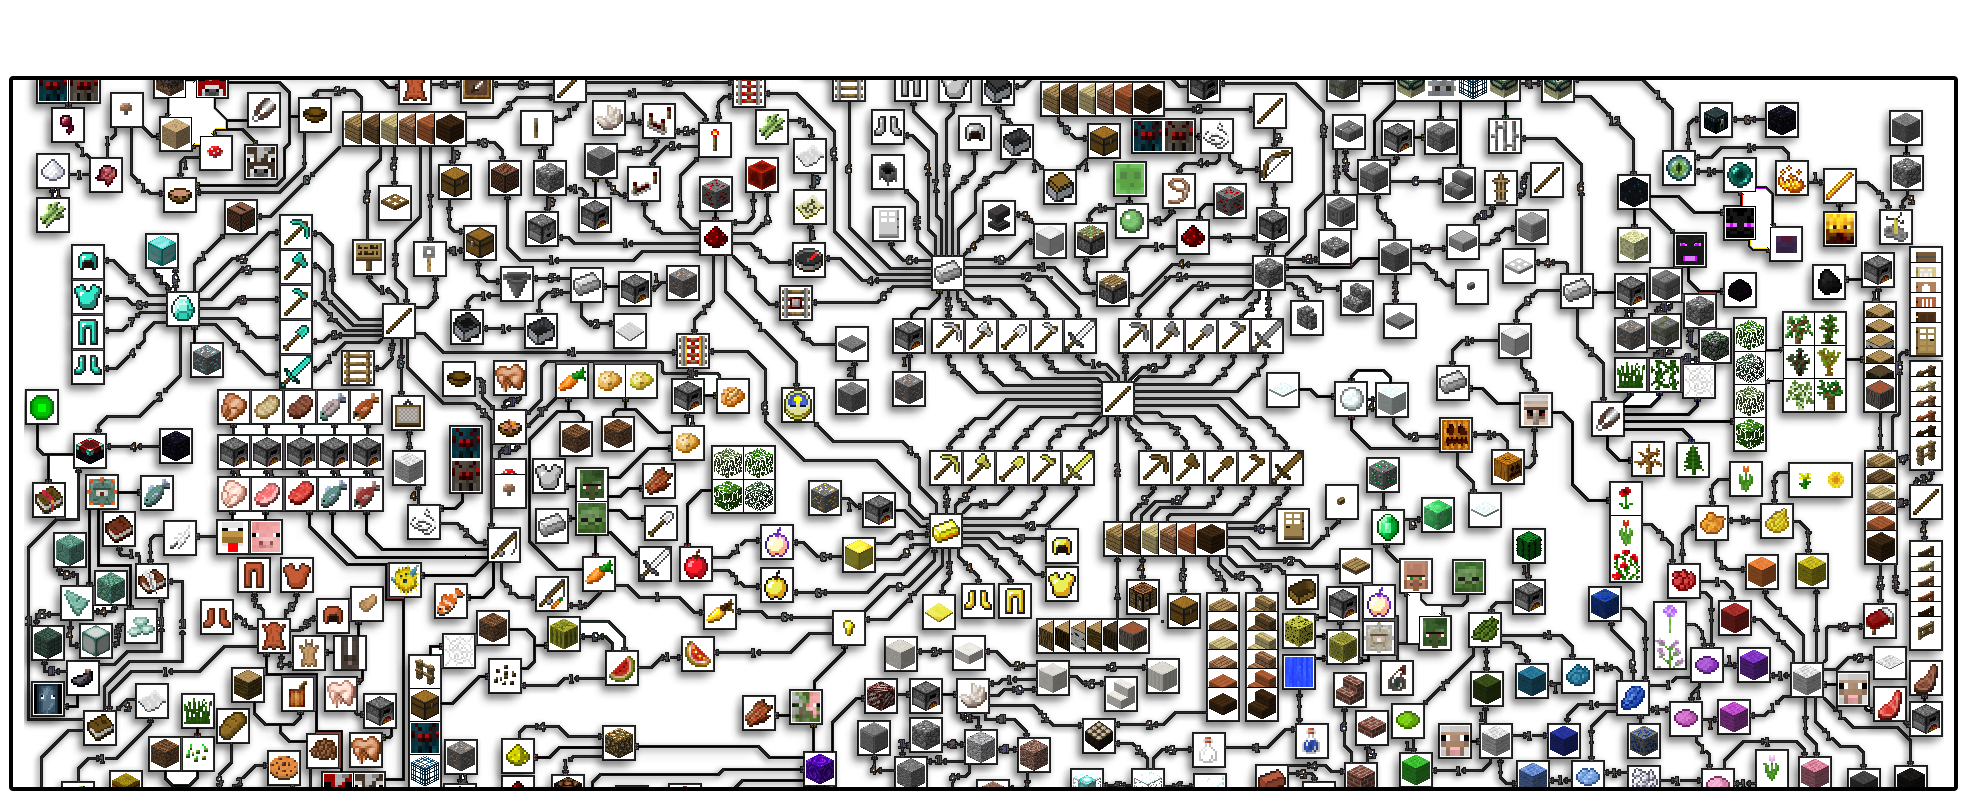
\includegraphics[width=0.9\textwidth]{./assets/item_hierarchy_final.png}
        \caption{\small{A subset of the Minecraft item hierarchy (totaling 371
        unique items). Each node is a unique Minecraft item, block, or non-player character, and a directed edge between two nodes denotes that
        one is a prerequisite for another. Each item presents is own unique
        set of challenges, so coverage of the full hierarchy by one player
        takes several hundred hours.}}
        \label{fig:hierarchicality}
    \end{center}
    \vspace{-19pt}
\end{figure}

Minecraft is a compelling domain for the development of reinforcement and imitation learning methods because of the unique challenges it presents: Minecraft is a 3D, first-person, open-world game centered around the gathering of resources and creation of structures and items. 
Notably, the procedurally-generated world is composed of discrete blocks that allow modification; over the course of gameplay, players change their surroundings by gathering resources (such as wood from trees) and constructing structures (such as shelter and storage).
Since Minecraft is an embodied domain and the agent's surroundings are varied and dynamic, it presents many of the same challenges as real-world robotics domains. 
Therefore, solutions created for this competition are a step toward applying these same methods to real-world problems.

Furthermore, there is existing research interest in Minecraft. 
With the development of Malmo~\cite{johnson2016malmo}, a simulator for Minecraft, the environment has garnered great research interest:
many researchers~\cite{oh2016control,shu2017hierarchical,tessler2017deep} have leveraged Minecraft's massive hierarchality and expressive power as a simulator to make great strides in language-grounded, interpretable multi-task option-extraction, hierarchical lifelong learning, and active perception. 
However, much of the existing research utilizes toy tasks in Minecraft, often restricted to 2D movement, discrete positions, or artificially confined maps unrepresentative of the intrinsic complexity that human players typically face. 
These restrictions reflect the difficulty of the domain, the challenge of coping with fully-embodied human state- and action-spaces, and the complexity exhibited in optimal human policies. 

Our competition and the utilization of the large-scale \minenet-v0 dataset of human demonstrations will serve to catalyze research on this domain in two ways: (1) our preliminary results indicate that through imitation learning, basic reinforcement learning approaches can finally deal directly with the full, unrestricted state- and action-space of Minecraft;  and (2) due to the difficult and crucial research challenges exhibited on the primary competition task, \texttt{ObtainDiamond}, we believe that the competition will bring work on the Minecraft domain to the fore of sample-efficient reinforcement learning research.

